\documentclass[aspectratio=169,10pt]{beamer}

\usetheme{metropolis}
\usepackage{appendixnumberbeamer}

\usepackage{booktabs}
\usepackage[scale=2]{ccicons}

\usepackage{pgfplots}
\usepgfplotslibrary{dateplot}

\usepackage{xspace}
\newcommand{\themename}{\textbf{\textsc{metropolis}}\xspace}

\usepackage{graphicx}

% Uses Ethereum colorful logo instead of bullet, for all item levels.
\defbeamertemplate{itemize item}{image}{\large
\includegraphics[height=1.6ex]{images/bullet}}
\defbeamertemplate{itemize subitem}{image}{\large
\includegraphics[height=1.6ex]{images/bullet}}
\defbeamertemplate{itemize subsubitem}{image}{\large
\includegraphics[height=1.6ex]{images/bullet}}
\setbeamertemplate{itemize item}[image]
\setbeamertemplate{itemize subitem}[image]
\setbeamertemplate{itemize subsubitem}[image]


% Sets the template background image for all the slides.
% Change opacity here.
\setbeamertemplate{background}{%
	\begin{tikzpicture}[remember picture,overlay]
		\node[at=(current page.center),opacity=0.2]{
			
\includegraphics[width=\paperwidth,height=\paperheight]{images/bg}
		};
	\end{tikzpicture}
}


% Sets the color theme.
% Change here for light theme.
% `sectionpage=none` removes slide between sections.
%\metroset{background=dark,sectionpage=none}
%\metroset{background=light}
\metroset{background=dark}
\usebeamercolor[fg]{normal text}

% Sets the footer `devcon iv` on the bottom right.
% Change `devcon iv` text color here.
\setbeamercolor{frame footer}{fg=gray}
\setbeamertemplate{frame footer}{devcon iv}

% If you use the light theme, you need to manually change the
% icons to `_black`.
% Change your GitHub username here.
\setbeamertemplate{github}{
  \normalsize
\includegraphics[height=1.6ex]{icons/github_white}
  mycodername
}
% Change your email here.
\setbeamertemplate{email}{
  \normalsize
\includegraphics[height=1.6ex]{icons/email_white}
  me@email.org
}
% Change your twitter account here.
\setbeamertemplate{twitter}{
  \normalsize
\includegraphics[height=1.6ex]{icons/twitter_white}
  myinternetname
}

% Remove here any contact you do not want to show.
\setbeamertemplate{contact}{
  \vspace*{1mm}
  \usebeamertemplate{github}\\
  \usebeamertemplate{email}\\
  \usebeamertemplate{twitter}
}

% Change presentation data here.
\title{{\Huge This is the name\\of my talk}}
\author{{\large Firstname Lastname}}
% Change date here.
% Empty date removes it from the frame.
% \date{\today} prints compilation date.
%Otherwise prints content.
\date{} %\date{\today}
\institute{{\large Companyname}}
% Sets the Ethereum/devcon logo on the upper left.
\titlegraphic{\vfill
\includegraphics[height=1.2cm]{images/devcon}}

\begin{document}

{
\setbeamertemplate{background}{%
	\begin{tikzpicture}[remember picture,overlay]
		\node[at=(current page.center),opacity=0.1]{
			
\includegraphics[width=\paperwidth,height=\paperheight]{images/bg}
		};
		\node[opacity=0.9] at (11.5,-2) {
			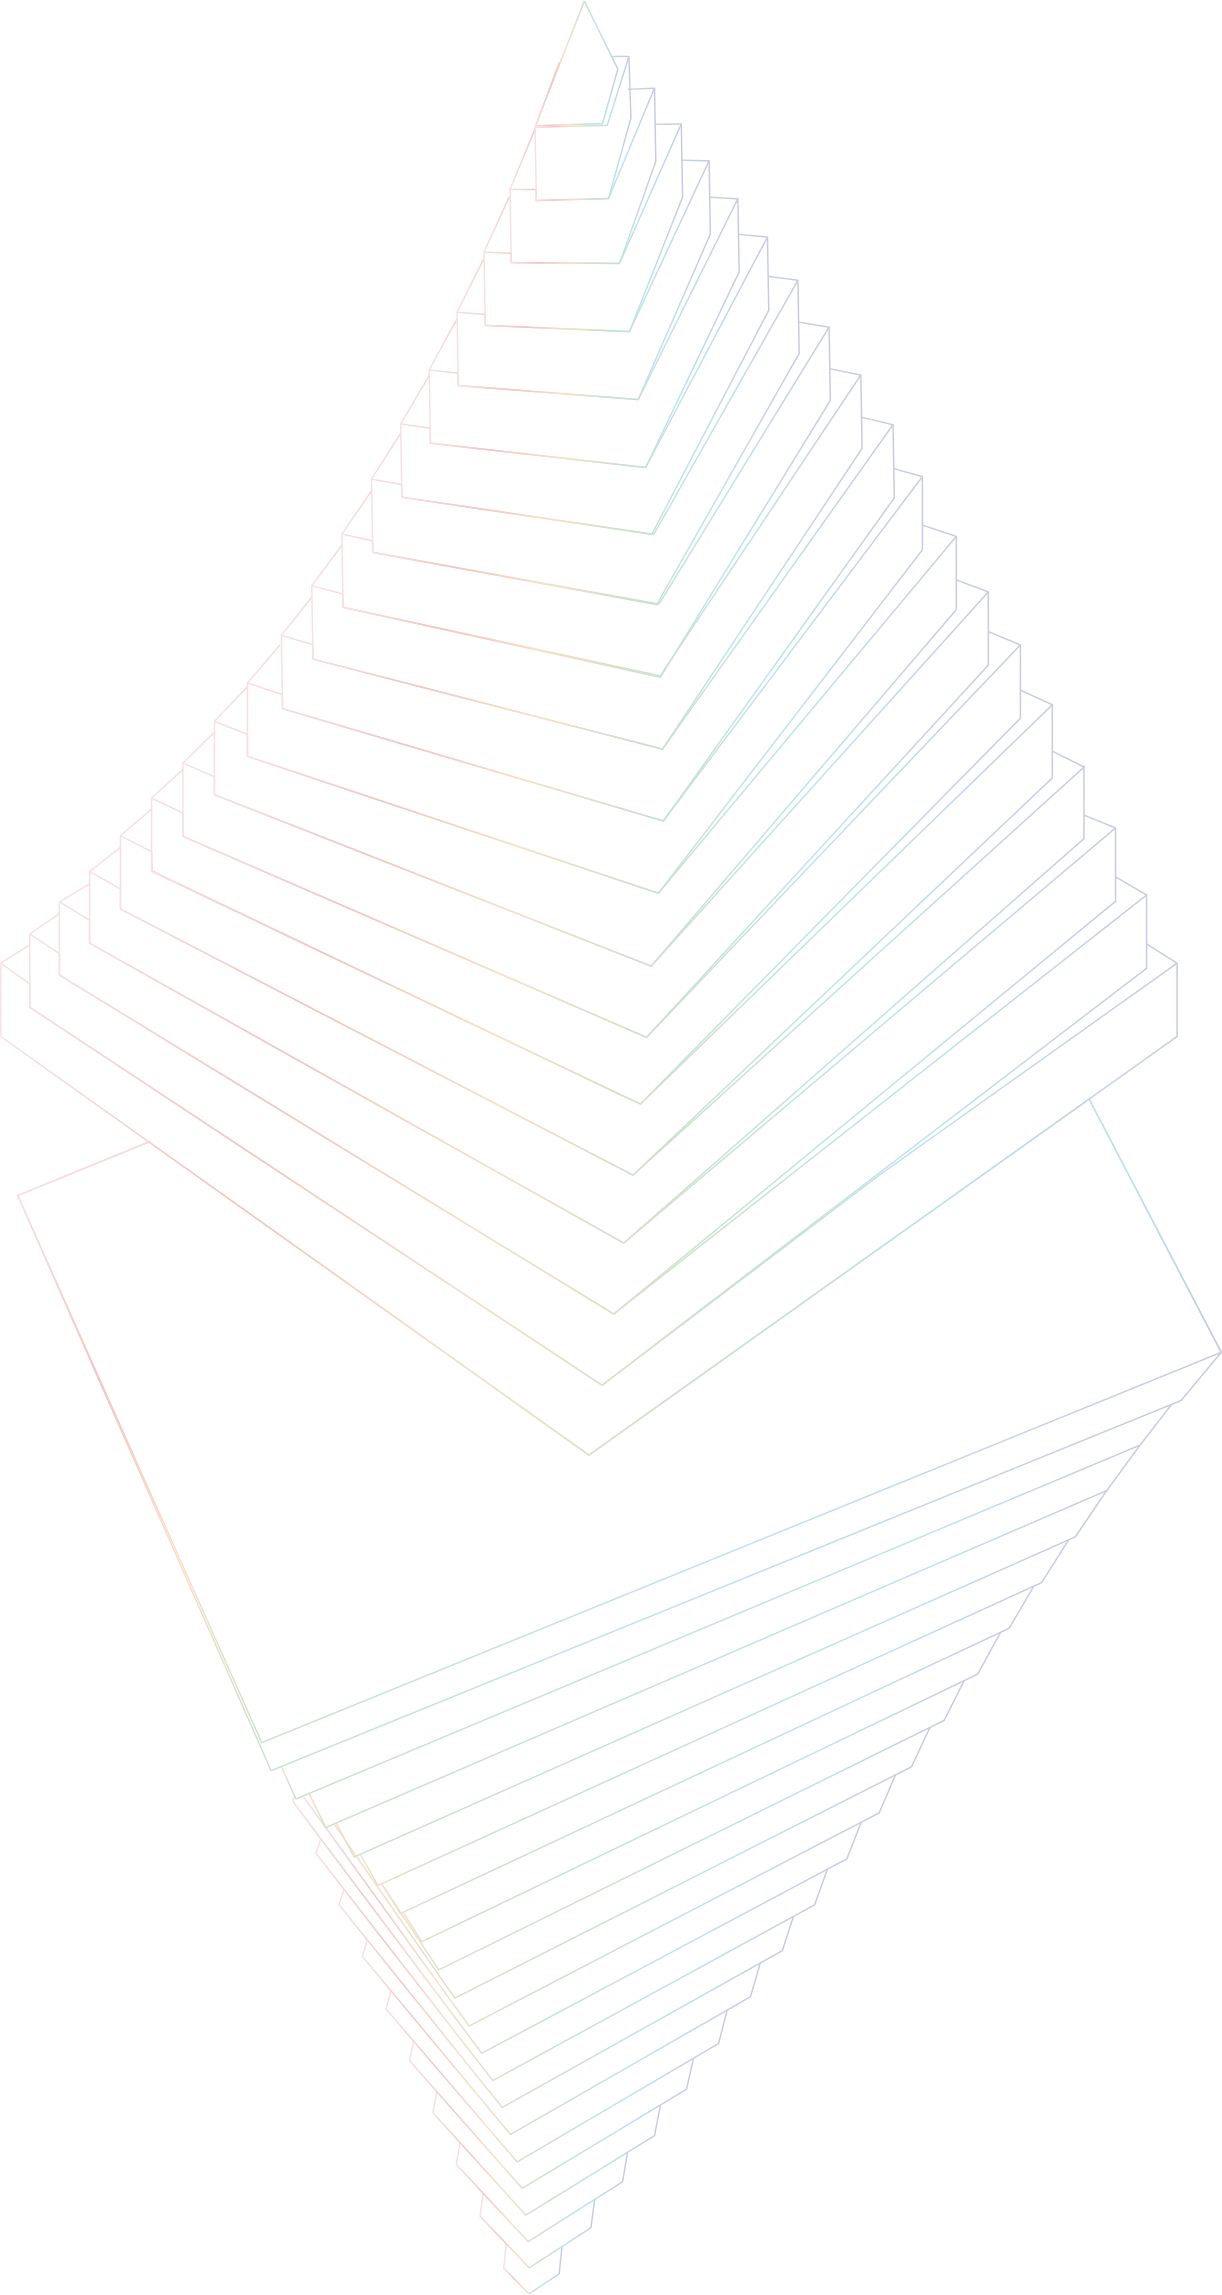
\includegraphics[keepaspectratio,scale=0.24]{images/title_logo}
		};
	\end{tikzpicture}
}
\begin{frame}
\maketitle
\end{frame}
}

\begin{frame}{This is a slide with a large block of text}
\begin{block}{}
Lorem ipsum dolor sit amet, consectetur adipiscing elit,
sed do eiusmod tempor incididunt ut labore et dolore magna
aliqua. Ut enim ad minim veniam, quis nostrud exercitation
ullamco laboris nisi ut aliquip ex ea commodo consequat.

Duis aute irure dolor in reprehenderit in voluptate velit
esse cillum dolore eu fugiat nulla pariatur. Excepteur
sint occaecat cupidatat non proident, sunt in culpa qui
officia deserunt mollit anim id est laborum.
\end{block}
\end{frame}

\begin{frame}{This is a slide with bulleted text}
\begin{itemize}
\item Lorem ipsum dolor sit amet, consectetur adipiscing elit, sed do eiusmod
	tempor incididunt ut labore et dolore magna aliqua.
	\begin{itemize}
	\item Ut enim ad minim veniam, quis nostrud exercitation.
	\end{itemize}
\item Duis aute irure dolor in reprehenderit in voluptate velit esse cillum
	dolore eu fugiat nulla pariatur.
\item Excepteur sint occaecat cupidatat non proident, sunt in culpa qui officia
	deserunt mollit anim id est laborum.
\end{itemize}
\end{frame}

\begin{frame}[standout]
Here's a really important statement that you want to emphasize.
\end{frame}

\section{Elements}

\begin{frame}[fragile]{Typography}
\begin{verbatim}The theme provides sensible defaults to \emph{emphasize}
text, \alert{accent} parts or show \textbf{bold} results.\end{verbatim}

\begin{center}becomes\end{center}

The theme provides sensible defaults to \emph{emphasize} text,
\alert{accent} parts or show \textbf{bold} results.
\end{frame}

\begin{frame}{Font feature test}
  \begin{itemize}
    \item Regular
    \item \textit{Italic}
    \item \textsc{Small Caps}
    \item \textbf{Bold}
    \item \textbf{\textit{Bold Italic}}
    \item \textbf{\textsc{Bold Small Caps}}
    \item \texttt{Monospace}
    \item \texttt{\textit{Monospace Italic}}
    \item \texttt{\textbf{Monospace Bold}}
    \item \texttt{\textbf{\textit{Monospace Bold Italic}}}
  \end{itemize}
\end{frame}

\begin{frame}{Lists}
  \begin{columns}[T,onlytextwidth]
    \column{0.33\textwidth}
      Items
      \begin{itemize}
        \item Milk \item Eggs \item Potatoes
      \end{itemize}

    \column{0.33\textwidth}
      Enumerations
      \begin{enumerate}
        \item First, \item Second and \item Last.
      \end{enumerate}

    \column{0.33\textwidth}
      Descriptions
      \begin{description}
        \item[PowerPoint] Meeh. \item[Beamer] Yeeeha.
      \end{description}
  \end{columns}
\end{frame}
\begin{frame}{Animation}
  \begin{itemize}[<+- | alert@+>]
    \item \alert<4>{This is\only<4>{ really} important}
    \item Now this
    \item And now this
  \end{itemize}
\end{frame}
\begin{frame}{Figures}
  \begin{figure}
    \newcounter{density}
    \setcounter{density}{20}
    \begin{tikzpicture}
      \def\couleur{alerted text.fg}
      \path[coordinate] (0,0)  coordinate(A)
                  ++( 90:5cm) coordinate(B)
                  ++(0:5cm) coordinate(C)
                  ++(-90:5cm) coordinate(D);
      \draw[fill=\couleur!\thedensity] (A) -- (B) -- (C) --(D) -- cycle;
      \foreach \x in {1,...,40}{%
          \pgfmathsetcounter{density}{\thedensity+20}
          \setcounter{density}{\thedensity}
          \path[coordinate] coordinate(X) at (A){};
          \path[coordinate] (A) -- (B) coordinate[pos=.10](A)
                              -- (C) coordinate[pos=.10](B)
                              -- (D) coordinate[pos=.10](C)
                              -- (X) coordinate[pos=.10](D);
          \draw[fill=\couleur!\thedensity] (A)--(B)--(C)-- (D) -- cycle;
      }
    \end{tikzpicture}
    \caption{Rotated square from
    \href{http://www.texample.net/tikz/examples/rotated-polygons/}{texample.net}.}
  \end{figure}
\end{frame}
\begin{frame}{Tables}
  \begin{table}
    \caption{Largest cities in the world (source: Wikipedia)}
    \begin{tabular}{@{} lr @{}}
      \toprule
      City & Population\\
      \midrule
      Mexico City & 20,116,842\\
      Shanghai & 19,210,000\\
      Peking & 15,796,450\\
      Istanbul & 14,160,467\\
      \bottomrule
    \end{tabular}
  \end{table}
\end{frame}
\begin{frame}{Blocks}
  Three different block environments are pre-defined and may be styled with an
  optional background color.

  \begin{columns}[T,onlytextwidth]
    \column{0.5\textwidth}
      \begin{block}{Default}
        Block content.
      \end{block}

      \begin{alertblock}{Alert}
        Block content.
      \end{alertblock}

      \begin{exampleblock}{Example}
        Block content.
      \end{exampleblock}

    \column{0.5\textwidth}

      \metroset{block=fill}

      \begin{block}{Default}
        Block content.
      \end{block}

      \begin{alertblock}{Alert}
        Block content.
      \end{alertblock}

      \begin{exampleblock}{Example}
        Block content.
      \end{exampleblock}

  \end{columns}
\end{frame}
\begin{frame}{Math}
  \begin{equation*}
    e = \lim_{n\to \infty} \left(1 + \frac{1}{n}\right)^n
  \end{equation*}
\end{frame}
\begin{frame}{Line plots}
  \begin{figure}
    \begin{tikzpicture}
      \begin{axis}[
        mlineplot,
        width=0.9\textwidth,
        height=6cm,
      ]

        \addplot {sin(deg(x))};
        \addplot+[samples=100] {sin(deg(2*x))};

      \end{axis}
    \end{tikzpicture}
  \end{figure}
\end{frame}
\begin{frame}{Bar charts}
  \begin{figure}
    \begin{tikzpicture}
      \begin{axis}[
        mbarplot,
        xlabel={Foo},
        ylabel={Bar},
        width=0.9\textwidth,
        height=6cm,
      ]

      \addplot plot coordinates {(1, 20) (2, 25) (3, 22.4) (4, 12.4)};
      \addplot plot coordinates {(1, 18) (2, 24) (3, 23.5) (4, 13.2)};
      \addplot plot coordinates {(1, 10) (2, 19) (3, 25) (4, 15.2)};

      \legend{lorem, ipsum, dolor}

      \end{axis}
    \end{tikzpicture}
  \end{figure}
\end{frame}
\begin{frame}{Quotes}
  \begin{quote}
    Veni, Vidi, Vici
  \end{quote}
\end{frame}

{%
\setbeamertemplate{frame footer}{My custom footer}
\begin{frame}[fragile]{Frame footer}
    \themename defines a custom beamer template to add a text to the footer. It can be set via
    \begin{verbatim}\setbeamertemplate{frame footer}{My custom footer}\end{verbatim}
\end{frame}
}

\begin{frame}{References}
  Some references to showcase [allowframebreaks] \cite{knuth92,ConcreteMath,Simpson,Er01,greenwade93}
\end{frame}

\section{Conclusion}

\begin{frame}[standout]
  Questions?
\end{frame}

\appendix

\begin{frame}[fragile]{Backup slides}
  Sometimes, it is useful to add slides at the end of your presentation to
  refer to during audience questions.

  The best way to do this is to include the \verb|appendixnumberbeamer|
  package in your preamble and call \verb|\appendix| before your backup slides.

  \themename will automatically turn off slide numbering and progress bars for
  slides in the appendix.
\end{frame}

\begin{frame}[allowframebreaks]{References}

  \bibliography{template}
  \bibliographystyle{abbrv}

\end{frame}

\end{document}
